\documentclass[conference]{IEEEtran}
\IEEEoverridecommandlockouts
% The preceding line is only needed to identify funding in the first footnote.
% If that is unneeded, please comment it out.
%\usepackage[backend=bibtex,style=verbose-trad2]{biblatex}

\usepackage{adjustbox}
\usepackage{algorithmic}
\usepackage{amsmath,amssymb,amsfonts}
%\usepackage[backend=bibtex,style=ieee]{biblatex}
%\usepackage{bookmark}
\usepackage{booktabs}
\usepackage{caption}
\usepackage{cite}
\usepackage{color}
\usepackage[inline]{enumitem}
\usepackage{float}
\usepackage[T1]{fontenc}
%\usepackage{fontspec}
\usepackage{footnote}
\usepackage{graphicx}
\usepackage[colorlinks=true,citecolor=blue]{hyperref}
\usepackage{inputenc}[utf8]
\usepackage{listings}
\usepackage{textcomp}
\usepackage[flushleft]{threeparttable}
\usepackage{subcaption}
\usepackage{xcolor}

\title{OpenCL Fast Fourier Transform%\\
%{\footnotesize \textsuperscript{*}Note: Sub-titles are not captured in Xplore 
% and should not be used}
%\thanks{Identify applicable funding agency here. If none, delete this.}
}

\pagenumbering{arabic}
\pagestyle{plain}

% Ensure decimal numbering in table  of contents
\renewcommand{\thesection}{\arabic{section}}
\renewcommand{\thesubsection}{\arabic{section}.\arabic{subsection}}
\renewcommand{\thesubsubsection}{\arabic{section}.\arabic{subsection}.\arabic{subsubsection}}

% ensure decimal numbering for sub sections
\makeatletter
\renewcommand{\@seccntformat}[1]{\csname the#1\endcsname.\quad}
\makeatother

% ------------------------------------------------------------------------%
% Proper Python Syntax Highlighting                                       %
% Author: redmode
% https://tex.stackexchange.com/questions/83882/how-to-highlight-python   %
% -syntax-in-latex-listings-lstinputlistings-command#83883                %
% ----------------------------------------------------------------------- %

% Default fixed font does not support bold face
\DeclareFixedFont{\ttb}{T1}{txtt}{bx}{n}{8} % for bold
\DeclareFixedFont{\ttm}{T1}{txtt}{m}{n}{8}  % for normal

% Custom colors
\definecolor{deepblue}{rgb}{0,0,0.5}
\definecolor{deepred}{rgb}{0.6,0,0}
\definecolor{deepgreen}{rgb}{0,0.5,0}

% Python style for highlighting
\newcommand\pythonstyle{
	\lstset{
		language=Python,
		basicstyle=\ttm,
		showstringspaces=false,
		tabsize=4,
		aboveskip=0.2cm,
		belowskip=0.2cm,
		otherkeywords={self},             % Add keywords here
		keywordstyle=\ttb\color{deepblue},
		emph={MyClass,__init__},          % Custom highlighting
		emphstyle=\ttb\color{deepred},    % Custom highlighting style
		stringstyle=\color{deepgreen},
		frame=tb,                          % Any extra options here
		prebreak=\textbackslash,
		linewidth=8.85cm,
		breaklines=true,
	}
}

% Python environment
\lstnewenvironment{python}[1][] {
	\pythonstyle\lstset{#1}
}{}

% Python for inline
\newcommand\pythoninline[1]{{\pythonstyle\lstinline!#1!}}

% Python for external file
\newcommand\pythonexternal[2][]{{\pythonstyle\lstinputlisting[#1]{#2}}}

% ----------------------------------------------------------------------- %

% Bash style for highlighting
\newcommand\bashstyle{
	\lstset{
		language=Bash,
		basicstyle=\ttm,
		showstringspaces=false,
		tabsize=2,
		%commentstyle=itshape,
		aboveskip=0.2cm,
		belowskip=0.2cm,
		prebreak=\textbackslash,
		extendedchars=true,
		mathescape=false,
		% literate= {\$}{{\textcolor{blue}{\$}}}1 {&}{{\textcolor{blue}{\&}}}1 {/n}{{\textcolor{green}{\textbackslash n}}}1,
		linewidth=8.85cm,
		breaklines=true
	}
}

% Bash environment
\lstnewenvironment{bash}[1][] {
	\bashstyle\lstset{#1}
}{}

% Bash for inline
\newcommand\bashinline[1]{{\bashstyle\lstinline!#1!}}

% Bash for external file
\newcommand\bashexternal[2][]{{\bashstyle\lstinputlisting[#1]{#2}}}


% Python style for highlighting
\newcommand\cstyle{
	\lstset{
		language=c,
		basicstyle=\ttm,
		showstringspaces=false,
		tabsize=4,
		aboveskip=0.2cm,
		belowskip=0.2cm,
		otherkeywords={self},             % Add keywords here
		keywordstyle=\ttb\color{deepblue},
		emph={MyClass,__init__},          % Custom highlighting
		emphstyle=\ttb\color{deepred},    % Custom highlighting style
		stringstyle=\color{deepgreen},
		frame=tb,                          % Any extra options here
		prebreak=\textbackslash,
		linewidth=8.85cm,
		breaklines=true,
	}
}

% Python environment
\lstnewenvironment{clist}[1][] {
	\cstyle\lstset{#1}
}{}

% Python for inline
\newcommand\cinline[1]{{\cstyle\lstinline!#1!}}

% Python for external file
\newcommand\cexternal[2][]{{\cstyle\lstinputlisting[#1]{#2}}}

% ----------------------------------------------------------------------- %

\begin{document}

\begin{titlepage}
\begingroup
\centering
{\LARGE\bfseries OpenCL Fast Fourier Transform}

\vspace{1cm}

{\Large University of Amsterdam (UvA)}

\vspace{0.5cm}

{Corne Kenneth Lukken}

{\textit{Informatics Institute} \\
Amsterdam, Netherlands \\
info@dantalion.nl}

\vspace{4.0cm}

\begin{figure}[H]
	\centering
	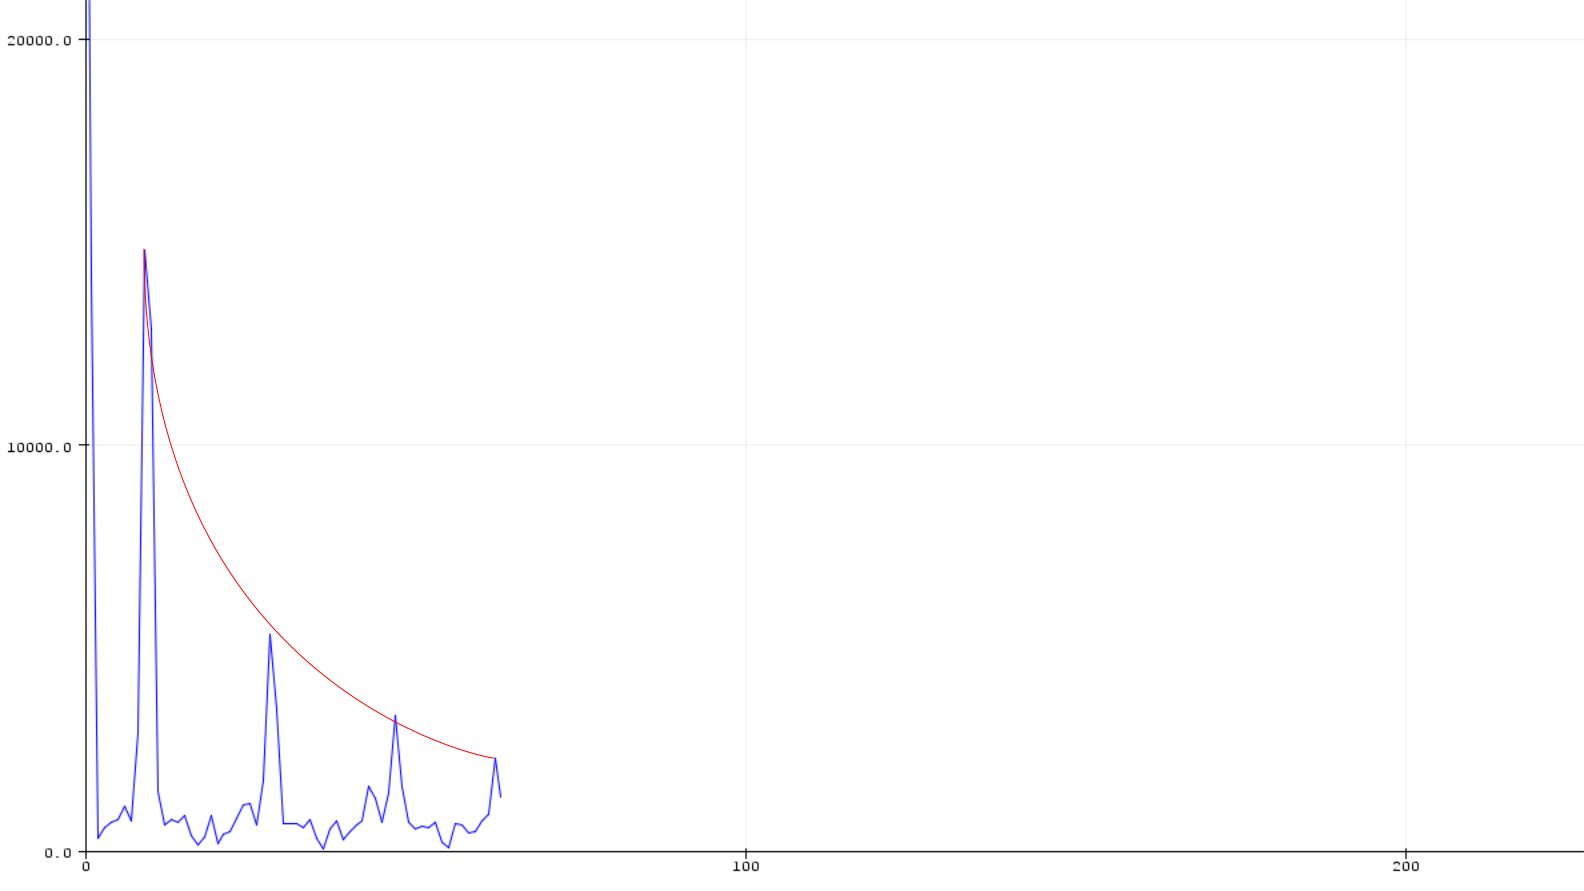
\includegraphics[width=0.7\textwidth]{resources/images/arduino-fft.png}
	\captionsetup{justification=centering}
	\caption{
		Output of embedded FFT library for which windowing \\
		and DC removal was implemented in previous work\cite{arduinofft}.
	}
\end{figure}

\vfill
\endgroup
\hfill
\begin{minipage}{0.3\textwidth}
\begin{flushright}
	
\includegraphics[width=\textwidth]{resources/images/uva-logo.png}
\end{flushright}
\end{minipage}
\end{titlepage}

\clearpage
\onecolumn

% Ensure black link color in table of contents
\hypersetup{
	linkcolor=black
}

\renewcommand{\contentsname}{CONTENTS}
\tableofcontents{}

\hypersetup{
	linkcolor=blue
}

\twocolumn

\addcontentsline{toc}{section}{\protect\numberline{}INTRODUCTION}
\section*{INTRODUCTION}
This introduction covers several different topics of which some might not be
interesting in terms of grading this project. Primary candidates for this
lesser interest are the section in which tools will be covered as well as a
section that breaks down the complicated landscape of HSA, SPIR-V, ROCm, clkv,
HIP, HCC and others\footnotemark[1]. Afterwards more relevant subjects such as
hardware platform and a breakdown of the chosen algorithm will be covered.
Finally, a summation of how various industry terms are interrupted or used is
covered at the end of this work \ref{term}.

\footnotetext[1]{Analyzing these subjects in depth is required to make well
informed decisions for the project. As these subjects need to be covered
regardless it was though it was best to write them down along the way. The
absolute explosion of standards and tools will likely cause a significant
portion of this project to be spent on investigating them.}

\subsection*{Accelerated Computing Landscape}

Current terminology, API's and standards make it undoubtedly clear that the
accelerated computing landscape is not reaching maturity any time soon. This is
further complicated by heterogeneous terminology which often overlaps with
accelerated computing. However, this vast landscape has benefits as well as it
currently introduces multiple methods of translating OpenCL\footnotemark[2]
unto an accelerator.

\footnotetext[2]{Some familiarity with terms mentioned in the title is
assumed.}

This work limits the types of accelerators to GPGPU's with both so called
discrete and integrated types covered. Additionally, possibilities of
heterogeneity are taken into account such as is made possible through the
Heterogeneous System Architecture (HSA) standard\cite{hsa1.2} among others.

\subsubsection*{Run-time's}

Before going into further details about heterogeneity firstly, some more
general GPGPU topics are discussed. Typically, code written in a programming
language such as \textit{C} or \textit{C++} is compiled using a compiler that
understands the target runtime. These compilers typically support a subset of
the language or expose certain libraries and functions\footnotemark[3]. In some
cases, primarily, 3D graphics applicationsn\footnotemark[4], a general purpose
compiler can be used and no specific runtime compiler is needed. The five most
common run-time's are \begin{enumerate*} \item OpenGL \item OpenCL \item
DirectX \item Vulkan \item CUDA \end{enumerate*}.

\footnotetext[3]{Functions are used to refer to programming even though
methods could be used as well. The term methods is reserved for more general
topics such as using it as a synonym for approach.}

\footnotetext[4]{The term application and program can be used interchangeably
throughout this work. It refers to a binary that can be executed.}

Of these only OpenCL and CUDA target compute applications all others are
primarily intended at 3D graphics, additional run-time's do exist such as HSA
but are typically targeted at specific types of computations different
than 3D graphics. What greatly complicates the understanding of the these
run-time's is that they require both software and hardware support. That is to
say the device requires a specific version of the runtime to be
implemented\footnotemark[5] as well as the software installed on the host.
Typically, the maximum supported version for a given application is the lowest
version of the device and the host software.

\footnotetext[5]{Sometimes these devices get upgraded to more recent runtime
versions through a firmware or bios update.}

Unfortunately, complications do not end here as multiple implementations of
different versions of software run-time's do exist. Sometimes multiple
run-time's are offered by the same vendor as well as not all these run-time's
being supported by all hardware offered by these vendors! Typically the
supported hardware is determined by a higher order driver, a kernel module in
the case of Linux. This driver subsequently implements one or more specific
versions of run-time's. This in term determines which run-time's are available
for a specific operating system and set of hardware.

The combination of kernel drivers, run-time's and tools is typically called a
\textit{stack}. Typical examples include the \textit{ROCm} or
\textit{AMDGPU-PRO} stacks both from AMD. In rare exceptions parts of these
stacks can be mixed and matches from different implementations but this
should never be assumed to be true. An example of such flexibility is the
ability to use the Mesa implementations of Vulkan and OpenGL while using the
ROCm stack.

Sometimes third-parties offer software stacks or run-time's for specific
sets of vendor hardware. An example of such a stack is \textit{Nouveau} which
is a reversed engineered software stack for Nvidia devices. In almost all cases
such a third-party software stack or runtime is open-source under a permissive
or copy-left license. Although vendor specific software is surprisingly
open-source in this field apart from Nvidia.

\subsubsection*{Intermediate Representation}

Sometimes compilers do not compile code directly into a executable and for some
run-time's such as OpenCL this is even impossible. Instead these compilers
generate a so called intermediate representation (IR) that often resembles
something close to assembly. Subsequently, this IR can be used to run using a
specific runtime. In the case of OpenCL this is achieved by reading the IR from
disc or a variable in the application currently being executed on the host.
Other run-time's typically offer a more static approach that does not require
reading or compiling code at run time\footnotemark[6].

\footnotetext[6]{This refers to the applications running state, not previously
mentioned run-time's such as Opencl or Vulkan.}

The major advantage of such an IR representation is that the target runtime can
be changed at any point in time and is decoupled from the programming language
and API's used to generate the IR. Additionally, it allows to more effectively
develop compiler optimizations assuming efforts are combined to improve the IR
backend.

Currently two major IR's for GPGPU's exist one being SPIR-V and the
other PTX. This work will focus mostly on SPIR-V as it allows translation of
OpenCL code unto a Vulkan runtime. Similar projects for PTX do exists as is the
case with GPUOCelot\cite{tired-manycore-architectures-ocelot} but typically are
no longer maintained. Additionally, some tools such as LLVM-SPIRV allow
bi-directional translation.

When an application is finally being run with a specific run-time, the
host executes a set of API calls that communicate with the driver. The
driver interprets these instructions and sends commands and data over a
communication bus between the host and device. Subsequently the device
interprets these commands and prepares execution\footnotemark[7]. The to be
executed set of instructions is called a \textit{kernel}. The actual
instructions being executed on the device are part of a so called Instruction
Set Architecture (ISA). This work does not go into explicit detail about
different ISA's unless it is relevant for reasoning about the performance of an
application.

\footnotetext[7]{What is actually being communicated between devices and host
is typically not known as it is not required by any run-time API to define how
this communication needs to happen. Only what behavior is expected when certain
calls are made.}

\subsubsection*{Heterogeneity}

One major research area for run-time's is in the field of heterogeneous
computing. Many organizations such as the HSA foundation, Khronos group and
AMD are working together to continuously improve standards such as OpenCL.
While OpenCL exists for quite some time now, the Heterogeneous System
Architecture (HSA) and ROCm stack are relatively new. This stack not only
implements OpenCL using HSA but also introduces several entirely new compilers
and frameworks to directly target HSA as a runtime. These frameworks are mainly
HIP and HCC were HIP allows to convert CUDA applications to a similar API that
targets a HSA runtime. Alternatively, HCC is able to target multiple so called
\textit{accelerator} modes including HIP but also C++ AMP or C++ Parallel STL.
Unfortunately, this ROCm stack has several limitations such as the deprecation
of HCC as of 2019 as well as only supporting GCN micro-architecture cards
(polaris 10, 11, vega 10, 11, 20). In addition, a representative from AMD has
confirmed that micro-architectures without an Instinct series card
(such as RDNA) will not get official ROCm support\cite{rocm-no-rdna}.

\section{FAST FOURIER TRANSFORM}

The fast fourier transform (FFT) is a fast algorithm for the discrete fourier
transform (DFT). This transforms complex data from the time domain to the
frequency domain in \textit{forward} mode or vice versa in \textit{reverse}
mode. In mathematics the reverse operation is called the inverse while the
terms \textit{forward} and \textit{reverse} are generally used by libraries.
Understanding how this transformation works can be quite hard to understand,
fortunately, 3Blue1Brown has an excellent visualization on the
matter\cite{fft-visualize}. The method with which the algorithm transforms 
complex numbers can be split into two components, firstly the discrete cosine
transform (DCT) and secondly, the discrete sine transform (DST). Separately
they both only transform real data but the two transforms can be combined in a
relatively straightforward manner to get the DFT algorithm.

All these combinations of operations allow for quite a large range of different
algorithms to still be called FFT. For this work the type of FFT considered is
one operated in forward mode with complex input data that applies the
transformation \textit{in-place}\footnotemark[8]. Here in-place implies that
the originally supplied input data will be modified to generate the output but
not necessarily that all output data can be read from the same memory addresses
as the input before the transformation.

\footnotetext[8]{If the target hardware allows it, for instance on GPGPU's
this is not trivially true.}

Apart from the type of FFT operation many different algorithms exist with
different computational complexities. Generally, algorithms that are more
restrictive to the input data are faster. Examples of such algorithms include
Cooley-Tukey\cite{Cooley1965} and Good-Thomas\cite{good-thomas} here the amount
of input samples is required to be a power of two or the multiplication of two
co-primes respectively.

Arguably, Cooley-Tukey is the most common FFT algorithm and has an algorithmic
complexity of $\mathcal{O}(N\log N)$. The algorithms primary distinction is
that it operates by recursively splitting the input data into two, hence the
power of two input samples requirement. Furthermore, the number by which the
input data is split in FFT's is known as the \textit{radix}, therefor,
Cooley-Tukey is a radix-2 algorithm. Additionally so called mixed-radix
implementations exist that can use a variety of different radix factors to be
less restrictive on input data, this is contrarily to split-radix
implementations that use different radix factors but instead are still as
restrictive on input data. Finally, some implementation use $\sqrt{N}$ as radix
factor, these are known as four-step or six-step algorithms and are currently
the best known cache-oblivious algorithms\cite{fast-fourier-cache}.

For this work a special implementation of Cooley-Tukey will be used, where the
in-place reordering of data allows to implement the algorithm without
recursion. Getting around the recursive nature of the algorithm is believed to
be important for porting to OpenCL.

\subsection{Correctness}

The wide variety of algorithms gives rise to different results for the same
input data, further complicated by the existence of fast approximations to
FFT subexpressions such as $\sin{}$, $\cos{}$ and $\sqrt{}$. Such
approximations could introduce errors in the results when compared to
implementations that do not use them. To eliminate some of these complications,
all computations and input data will use 64 bit floating point numbers,
otherwise known as double precision.

In forward mode, arguably the primary purpose of the FFT algorithm is to
determine frequency components and their magnitude from the input data.
However, accurately determining the frequency becomes impossible with small a
number of samples as was visualized by 3Blue1Brown\cite{heisenburg-frequency}.
Proofing that the algorithm has computed the best possible results hence
becomes difficult. Instead this works aims to compare the output of existing
FFT libraries and evaluate if the result is within some margin of error from
this reference. For this work FFTW\cite{FFTW05} will be used as it arguably
one of the most common FFT libraries.

The margin of error that is tolerated depends on the exponent and the input
sample. For every element of the result at least the first three digits of the
mantissa need to be identical except for the first and last element were only
two digits of the mantissa are required. Furthermore, every exponent above
$-10^{250}$ and below $+10^{250}$ needs to match exactly for every element.
Granted, these tolerances might seem pretty loose but this is believed to match
the goals of the envisioned projects.

\subsection{Windowing}

As mentioned the FFT algorithm operates on a discrete number of input samples.
However, this input is typically sampled from continuous systems such as
microphones or RF receivers. This algorithm gets around mathematical problems
from interpolating between finite and continuous systems by virtually
mirroring the input data to the right and left of the actual samples. An
example of this is shown in figure \ref{fig:consampling}. Here the above graph
attempts to illustrate the continuous data were the samples are taken between
the black bars. In the graph below the actual input samples are mirrored from
left to right. The result is sudden jumps in amplitude between samples due to
the first and last sample of the input data not having the same amplitude.

\begin{center}
	\begin{figure}[H]
		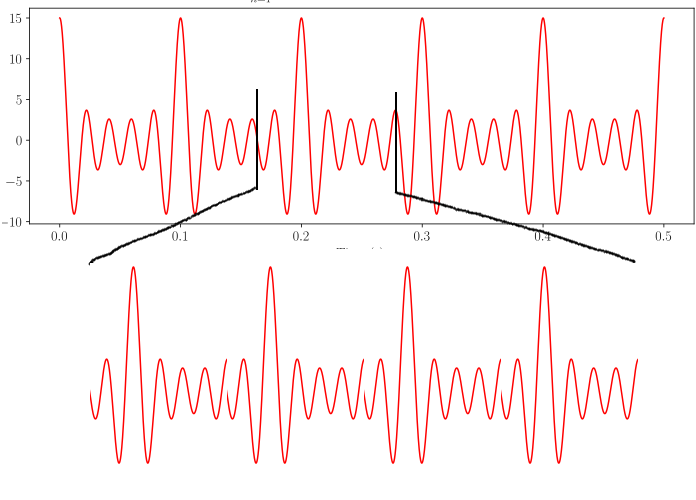
\includegraphics[width=0.5\textwidth]{resources/images/windowing-cc-by-sa-4-akantoe-wiki.png}
		\captionsetup{justification=centering}
		\caption{Example of sudden jumps in analyzed data due to amplitude
			differences in first and last sample. Original image by
			\href{https://commons.wikimedia.org/wiki/User:AkanoToE}{AkanoToE}
			licensed under CC-BY-SA 4.0}
		\label{fig:consampling}
	\end{figure}
\end{center}

If an FFT were to be applied to this data than the resulting FFT would show
incorrect results. To resolve these issues so called windowing functions are
applied to the input data prior to performing the FFT. These functions push
the amplitudes of samples at the start and end together in a smooth
transition. However, since all the inputs samples are now pushed towards the
same amplitude the resulting FFT loses accuracy in the actual amplitude of a
signal as well reducing the dynamic range. Therefor, windowing functions
essentially perform a balancing act between the ability to distinguish
individual signals close in frequency and the total dynamic range. As a result
different windowing functions are for different applications.

Since a windowing function is so essential for getting good results from the
FFT it is arguably part of the required computation. In this work the Nutall
windowing function will be applied to the input data as it has among the
highest dynamic range as well as good signal distinction. However, it has
high mathematical complexity as well. For comparison arguably the most common
windowing function is called Hann and has four terms while Nutall is a ten
term function. An overview of windowing functions is shown in
figure \ref{fig:windowingfuncs}.

\begin{center}
	\begin{figure}[H]
		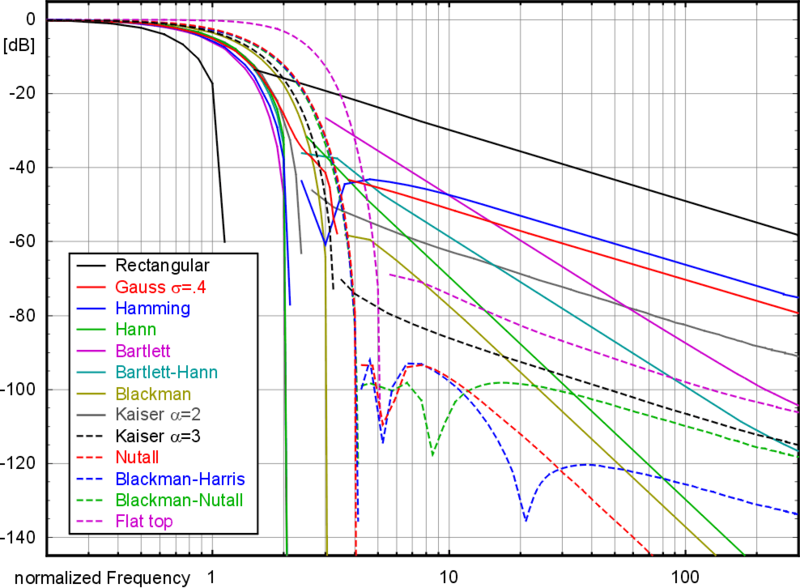
\includegraphics[width=0.5\textwidth]{resources/images/Window-function.png}
		\captionsetup{justification=centering}
		\caption{Different windowing functions their properties illustrated by
			\href{https://en.wikipedia.org/wiki/User:Marcel\_M\%C3\%83\%C2\%BCller}{MarcelMAller}
			licensed under CC-BY-SA 3.0}
		\label{fig:windowingfuncs}
	\end{figure}
\end{center}

Here dipping of the line from left to right shows how wide individual signals
will be, while the slope from right to left indicates the noise floor
corresponding to the dynamic range.

\subsection{Magnitude}

As mentioned windowing functions help balance properties such as the accuracy
of the measured amplitude. However, after the FFT is performed one more step is
required to determine this amplitude correctly. This final steps converts the
complex numbers from the FFT result into magnitudes. This is done by measuring
the distance from the center of the complex plane up to the point. In this
work the final \textit{complex to magnitude} is also considered as part of the
computation.

% \section*{TOOLS}

\section{Experimental Setup}

The goal of this work is to provide a real-time algorithm for the complete
computation of windowing, FFT and magnitude calculations. In this work
real-time implies that the entire computation must be finished in less than
16.66 milliseconds as a result a graphical representation of the computation
could than be maintained at 60 frames per second (fps). Any optimization is
allowed as long as the required accuracy relative to FFTW is maintained.
Additionally,

The computations required to perform this calculations are heavily depended
on the number of input samples. Therefor, the implementations are evaluated at
a variety of so called \textit{bin} sizes were the bin size corresponds to the
number of input samples. For this a collection of different input files from
sigidwiki\cite{sigidwiki} will be used for performance measurements. This
signal identification archive contains both audio and in-phase quadrature (IQ)
files that both will be used for performance measurements. Here audio files
will only contain real data and will be padded with zero for the imaginary
values while IQ data already contains imaginary values.

All input files will be stored as WAV files using 64 bit floats and converted
to csv to simplify the parsing. The amount of different input files will be
relatively limited as it should have no measurable impact on the performance.
Any mismatch between the sample rate of the input file and the currently
evaluated bin size will be resolved by a crude\footnotemark[9] decimation step.
The set of input files along with their attributes is shown in
table \ref{table:files}. Please note that the sample rate refers to the sample
rate after downconversion and does not correspond to the frequency of
transmission / reception.

\footnotetext[9]{Crude in the sense that actual downsampling typically also
consists of a lowpass filter.}

\begin{table}[h!]
	\caption{Input evaluation sizes}
	\label{table:files}
	\centering
	\begin{adjustbox}{width=0.5\textwidth}
		\begin{threeparttable}[]
			\begin{tabular}{llll}
				\toprule 
				\textbf{Name} & \textbf{Type} & \textbf{Sample rate (kHz)} &
				\textbf{Samples} \\
				\midrule
				xpa1 & real & 8 & 3140 \\
				xpa2 & real & 8 & 7990 \\
				jorn & real & 192 & 370650 \\
				acars & complex & 48 & 2408 \\
				flex & complex & 39.062 & 38598 \\
				ads-b & complex & 10000 & 502622 \\
				dvb-t & complex & 5333 & 2654207 \\
				\bottomrule
			\end{tabular}
			\begin{tablenotes}[para,flushleft]
				\centering List of input files and parameters used for
				performance evaluations.
			\end{tablenotes}
		\end{threeparttable}
	\end{adjustbox}
\end{table}

\section{Target Hardware}

The primary hardware used for performance evaluations is a desktop computer.
The specifications are shown in figure \ref{fig:inxihardware}. Other machines
might be evaluated as well primarily to compare the OpenCL performance across
different types of devices. These devices will be introduced separately later.

\begin{center}
	\begin{figure}[H]
		\bashexternal{resources/bash/inxi.sh}
		\captionsetup{justification=centering}
		\caption{Output of inxi showing both CPU and GPU hardware configuration}
		\label{fig:inxihardware}
	\end{figure}
\end{center}

As can be observed this machine has a GCN micro-architecture graphics card
and a Haswell series CPU. Both of these platforms allow the use open-source
OpenCL run-time's. Here the RX470 is supported through ROCm\cite{rocm} 3.3 and
the Haswell CPU is supported through beignet\cite{beignet} 1.3. However, it is
unlikely the OpenCL runtime will be used during this assignment.

\section{Roofline Model}

One of primary goals of this work is to use OpenCL to perform the desired
computations, however, it can still be beneficial to first model the
performance when using a regular CPU. This section reasons about the
arithmetic intensity for all three parts of the computation. Afterwards the
separate arithmetic intensities can be used to reason about the computation as
a whole.

This section will describe three different roofline models of which two for the
CPU and one for the GPU. By comparing these different models the potential
performance improvement over a CPU implementation for this specific hardware
can be theorized. All roofs in each model will be for 64 bit double precision
floating point arithmetic unless stated otherwise.

The CPU based models will be for sequential as well as parallel performance
using multiple roofs from scalar and vector arithmetic as well as modeling all
levels of memory. Each of these CPU roofs will be measured using
likwid bench\cite{likwid-bench} while the GPU will be measured using
gpumembench\cite{gpumembench}.

The first CPU roofline model is shown in figure \ref{fig:sequantialroofline}.
These models show each of the parts of the computation on a vertical dotted
line. As can be seen the magnitude computation has significantly lower
arithmetic intensity than the FFT and window functions. Luckily, the majority
of the computation will very likely be spent on the FFT as indicated by the
$\mathcal{O}()$ complexity.

In addition these roofs indicate that the FFT computation will not become
memory bound when using simple scalar instructions even when not utilizing
cache. However, if the FFT algorithm were to be vectorized the computation
could become memory bound without properly utilizing caches.

\begin{center}
	\begin{figure}[H]
		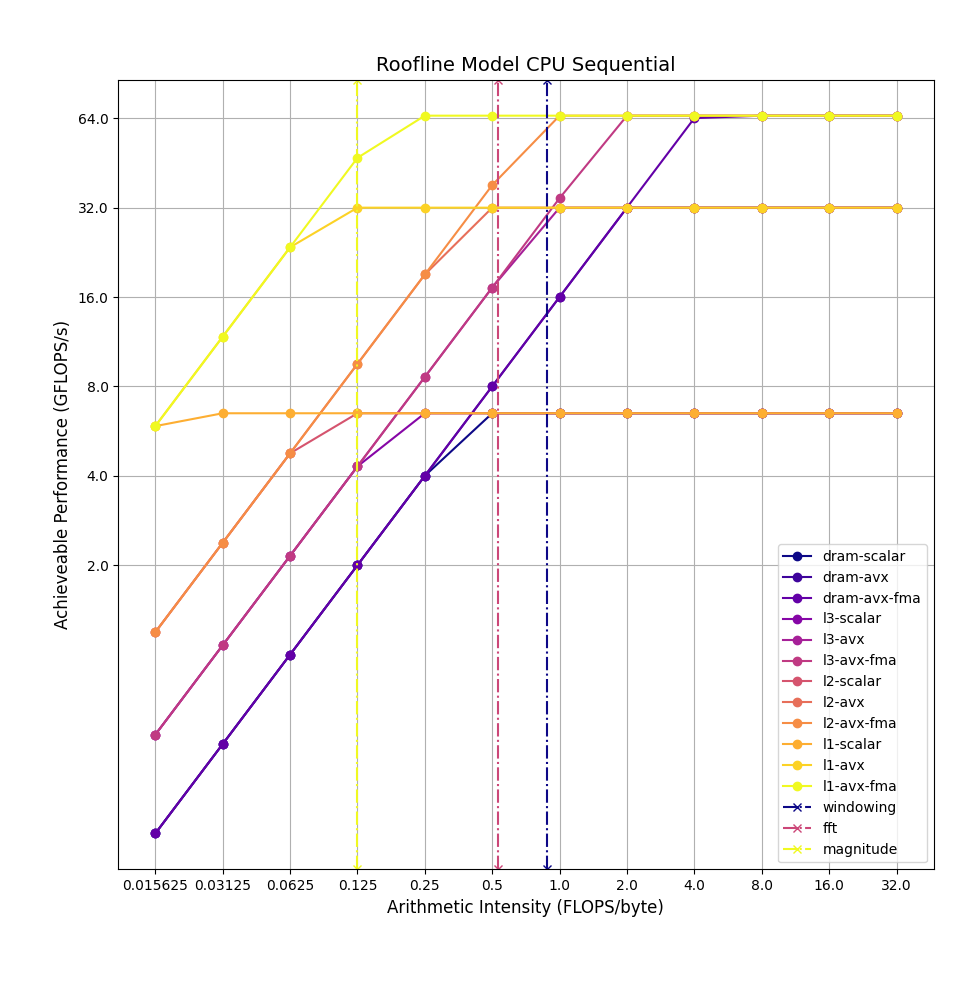
\includegraphics[width=0.5\textwidth]{resources/images/roof-seq-cpu.png}
		\captionsetup{justification=centering}
		\caption{Roofline model for single threaded CPU.}
		\label{fig:sequantialroofline}
	\end{figure}
\end{center}

The second roofline model shown in figure \ref{fig:mtroofline} is similar to
the first one except modeled using all four physical cores of the target
hardware. Just like the previous model these results represent actual
benchmarks and are not based on theoretical performance figures from
specifications.

This second figure clearly shows that optimizing cache utilizations is critical
to obtaining good performance for the FFT computation even when just using
scalar instructions. Additionally, the upper most roof indicates that up to
256 GFLOPS/s could achieved using FMA and L1 cache. However, reaching this
performance is unlikely as the size of input data can quickly grow beyond the
size of L1 cache and the majority of FFT computations involves complex
mathematical operations like $\sin{}$ and $\sqrt{}$.

\begin{center}
	\begin{figure}[H]
		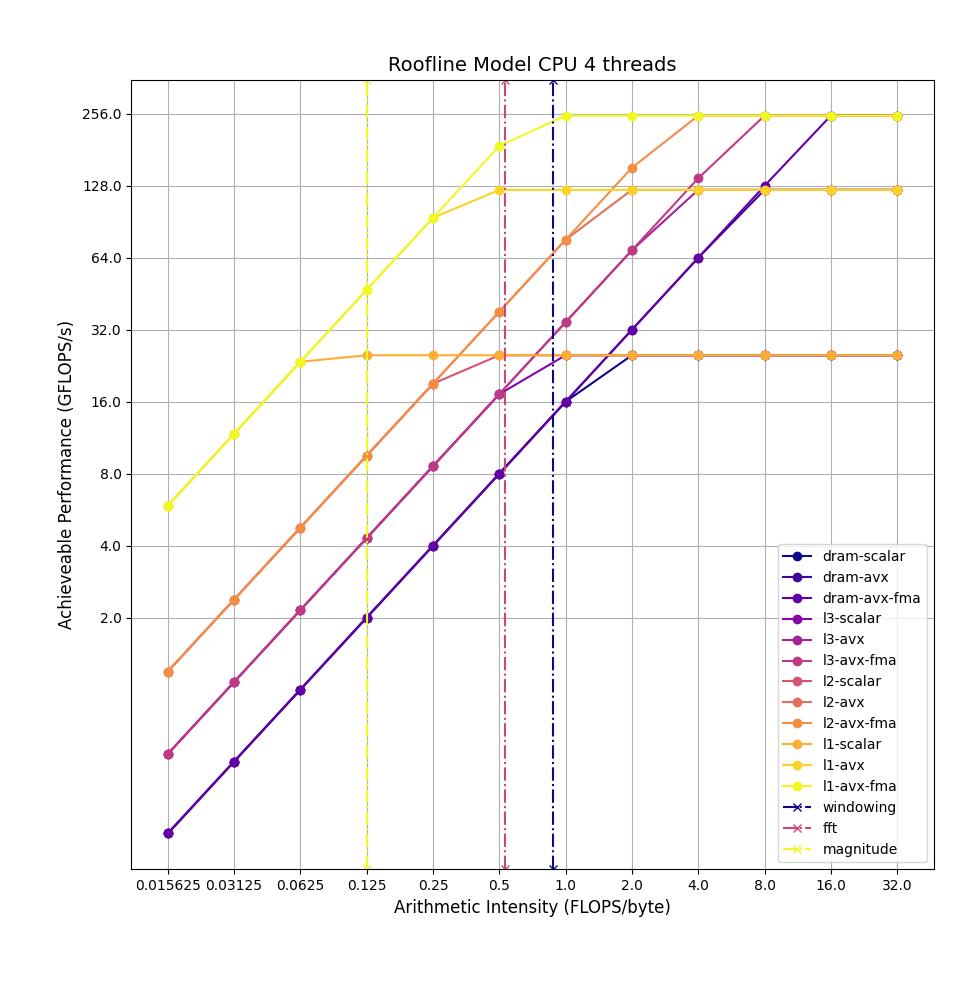
\includegraphics[width=0.5\textwidth]{resources/images/roof-mt4-cpu.png}
		\captionsetup{justification=centering}
		\caption{Roofline model for multi threaded CPU.}
		\label{fig:mtroofline}
	\end{figure}
\end{center}

When the roofline model is used for the GPU instead the memory visually appears
as less of a bottleneck as can be seen in figure \ref{fig:gpuroofline}.
However, this is not trivially true as the memory bandwidth shown in these
figures assumes that Compute Units (CU) access adjacent memory. If the memory
access patterns become erratic or strided the bandwidth can be reduced by a
factor of four in the case of 64 bit double precision floating point data. This
is because the memory bus on this specific GPU is 256 bits wide. Additionally,
the GPU roofline model shows the memory transfer speed at which data is
transfered between the host and device. This memory transfer takes often a
significant portion of the time to perform operations. One of the first steps
in eliminating this bottleneck is performing the windowing, FFT and magnitude
computations all on the GPU. This is because the data will only have to be
transfered at the start and end of all computations and individual parts can
reuse each others data.

\begin{center}
	\begin{figure}[H]
		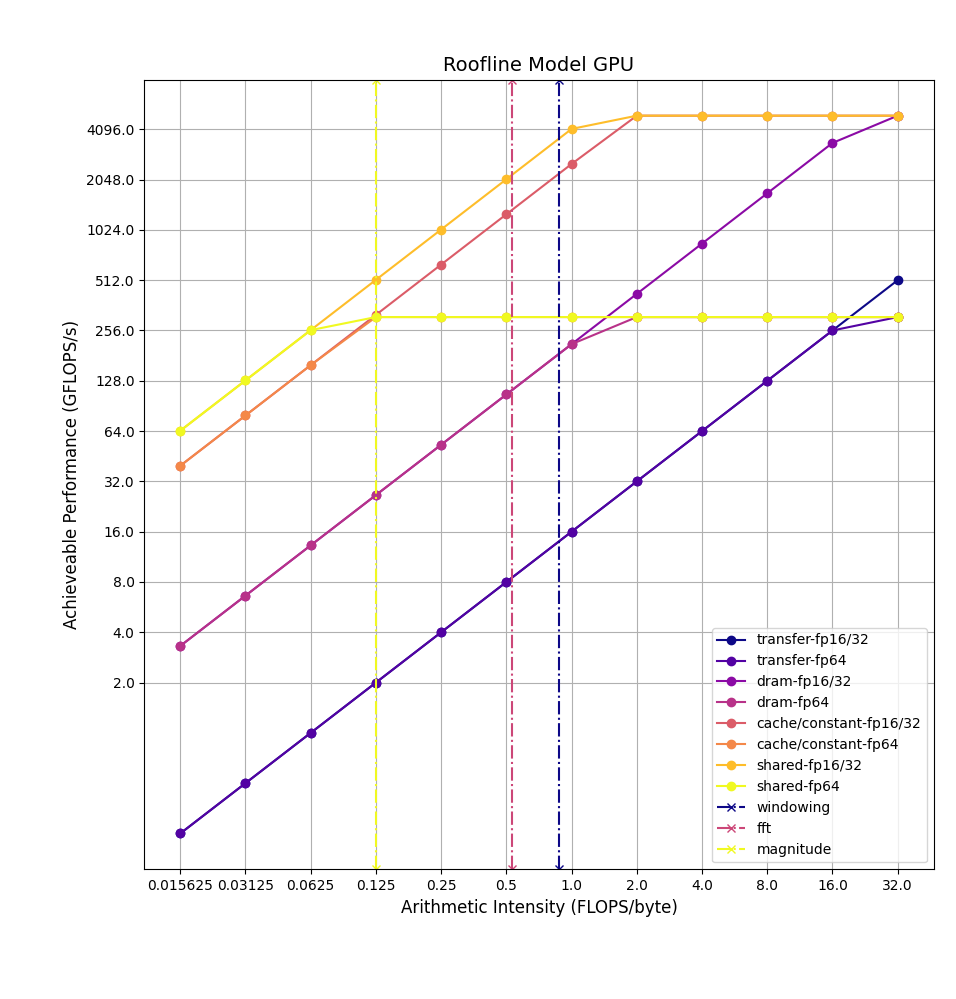
\includegraphics[width=0.5\textwidth]{resources/images/roof-gpu.png}
		\captionsetup{justification=centering}
		\caption{Roofline model for GPU.}
		\label{fig:gpuroofline}
	\end{figure}
\end{center}

\section{Basic OpenCL Implementation}

The first basic OpenCL implementation is based on adaptation of a Cooley-Tukey
reordered bit-reverse in-place algorithm\cite{arduinofft}. The conversion will
be a non-trivial process as both the bit-reversal and FFT algorithm itself have
many data dependencies and loop variables, therefor, the first basic
implementation will only use a single work-item for the bit-reversal and FFT.
The first implementation does not aim at achieving good performance but rather
at identifying dependencies that complicate the efficient use of the GPU.
Fortunately, both windowing and magnitude computations do not have similar data
dependencies and are trivially to parallelize with OpenCL. Combined with the
proportionally very small computation time it is unlikely that these two
sections will be revisited in this work.

The dependencies for the bit-reversal and remainder of the FFT are modeled
separately with potentially further dividing the FFT computation up into even
more smaller kernels in the future. This allows to identify that the vast
majority of computation time is spent on the remainder of the FFT and not on
the bit-reversal. However, improving of the bit-reversal might be done in the
future as it has been the topic of many interesting works
\cite{Rius1995,Karp1996,parreverse,Adikaram2014}.

Although this basic OpenCL implementation could be subjected to performance
evaluations it is believed better to first analyze for improvements rather than
evaluating such a poorly parallelized implementation. This basic implementation
is accessible in the source repository under the tag \textit{ard-ocl-basic}.

\subsection{Possible Optimizations}

The first OpenCL FFT kernel is shown in figure \ref{fig:basefftk}. This kernel
shows multiple variables that are depended on the current iterations of a loop
as well as previous values of these variables. These variables labeled
\textit{c1}, \textit{c2}, \textit{l1} and \textit{l2} are problematic as
computing them is depended on the previous loop iteration. Several different 
strategies to resolve these loop dependencies exist of which arguably the most
straightforward is having multiple work-items doing the same computation
redundantly. Obviously redundant computations are not ideal especially if the
amount of iterations will change per work-item.

\begin{center}
	\begin{figure}[H]
		\cexternal{resources/c/basic-fft.c}
		\captionsetup{justification=centering}
		\caption{First basic FFT kernel}
		\label{fig:basefftk}
	\end{figure}
\end{center}

Perhaps an unusual strategy for modern CPU and GPU architectures is the use of
a look-up table to access precomputed values. This strategy is often employed
on micro-controllers as these platforms do not have large differences in
latency between accessing memory or performing arithmetic operations. However,
since the amount of values for \textit{c1} and \textit{c2} is logarithmic with
the input size this becomes a valid strategy. In addition variables
\textit{l1} and \textit{l2} contain the values for powers of two making them
also easy to precompute. This allows to entirely eliminate the outermost loop
in the kernel.

A much larger problems is due to variables \textit{u1} and \textit{u2} as these
are also computed based on their previous values. Additionally, these are
depended on \textit{c1} and \textit{c2} resulting in the values varying for
each iteration of the eliminated outermost loop. These dependencies make it
impractical to store precomputed values of the entire range of values, however,
this might be the only practical method to obtain good performance. In
hindsight the effort spend porting of bit-reversed Cooley-Tukey FFT to OpenCL
was better spend porting another implementation with no variables that can only
be computed with variables from previous iterations.

\section{Lookup Implementation}

Regardless of complications a best effort is made to get the best possible
performance using the chosen implementation. However, manually creating such an
extremely large lookup table is impractical. Therefor, a small application is
written in C++ that will generate the source code for these tables. These
tables are generated up two $2^{21}$ which is enough for computing with an
input size of 2097152 elements or rather a bin size of 1048576. This limit is
due to the host to device and device to host memory transfers taken longer than
16.66 ms at this size.

The lookup implementation is implemented in two steps were some of the required
tables are kept on the host and others on the device. Firstly, for every power
of two of which the result is less than the number of input elements a kernel
is launched. These kernels can be launched in a loop where the parameters are
updated for each call based on values looked up in the tables. All calls use
the same queue as they depend on the results of previous calls. How these
kernels are launched is shown in figure \ref{fig:subfft}.

Subsequently, these kernels themselves also access a lookup table were 
The element to be accessed from this table is determined both from the current
power of two and the global id. However, this table is loaded from OpenCL
sources and build into the OpenCL program at runtime. This comes at a cost as
now roughly 300 MBytes of OpenCL source has to be loaded and compiled at
runtime resulting in a hight startup time. Nevertheless, this cost is not
counted towards the real-time requirements as it only occurs once during
program startup.

\begin{center}
	\begin{figure}[H]
		\cexternal{resources/c/submit-fft.c}
		\captionsetup{justification=centering}
		\caption{Looped FFT kernel submission}
		\label{fig:subfft}
	\end{figure}
\end{center}

When analyzing the performance of this implementation it can be observed that
the actual FFT can be performed faster than using FFTW for small input sizes.
The results for small input sizes is shown in figure \ref{fig:ardoclsmall}.
Additionally, it can be observed that the time to compute the window and
perform the copies is relatively constant for these small input sizes. Combined
the entire execution of \textit{ard-ocl} is still orders of magnitude slower
than using the CPU even though the windowing and magnitude are performed
sequentially. The largest bottleneck is the bit reversal as it is only executed
with a single work item.

\begin{center}
	\begin{figure}[H]
		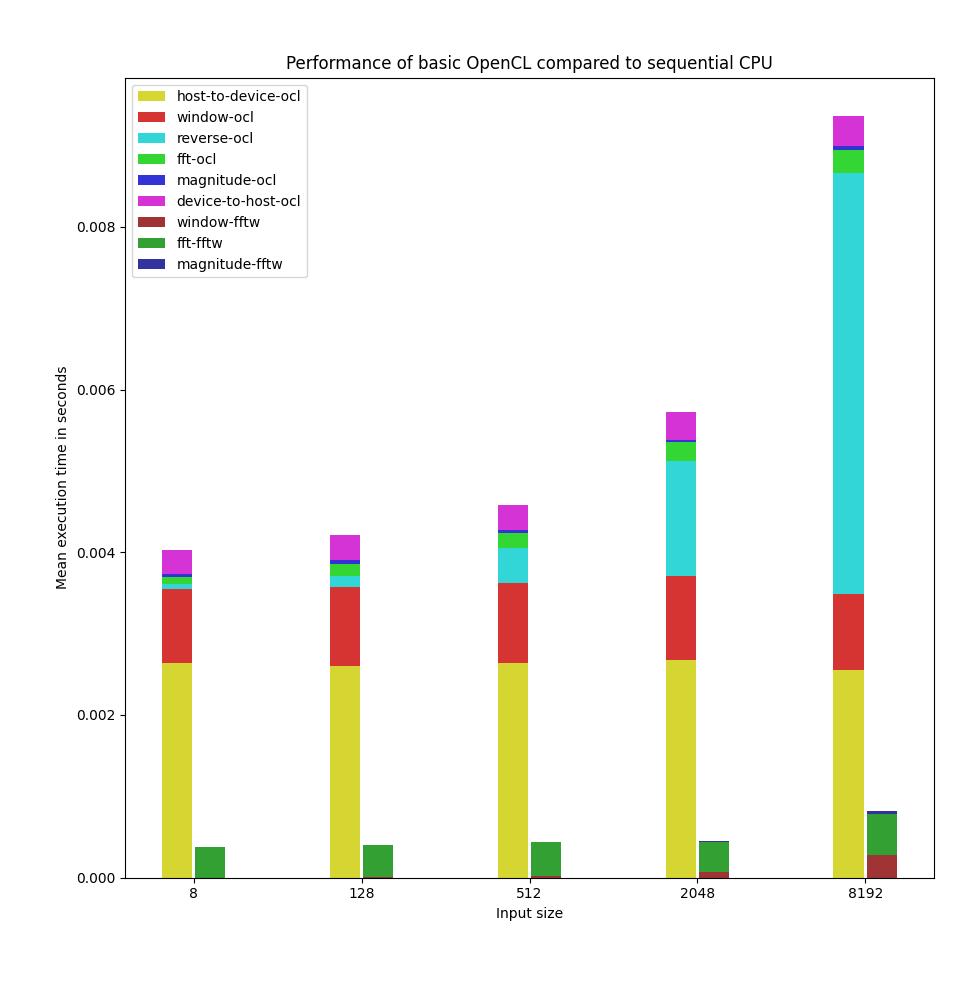
\includegraphics[width=0.5\textwidth]{resources/images/ard-ocl-low.png}
		\captionsetup{justification=centering}
		\caption{ard-ocl performance for small input sizes}
		\label{fig:ardoclsmall}
	\end{figure}
\end{center}

\begin{center}
	\begin{figure}[H]
		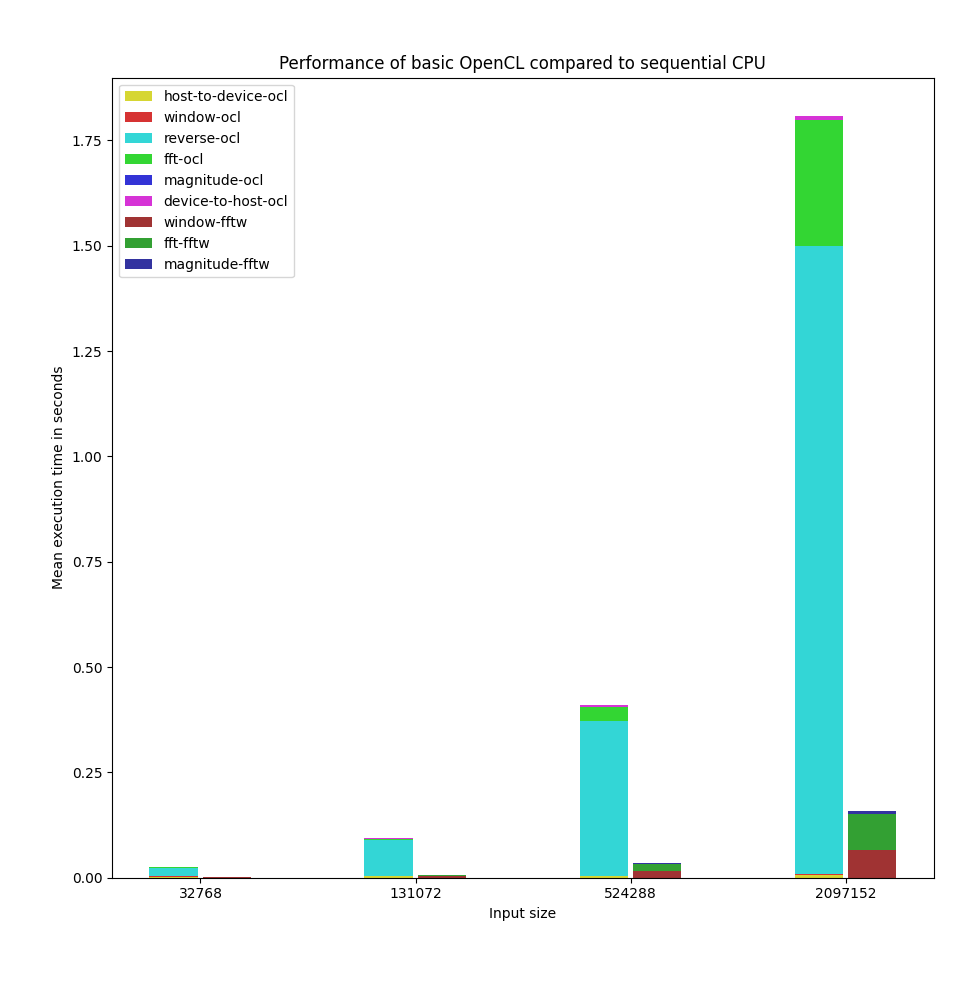
\includegraphics[width=0.5\textwidth]{resources/images/ard-ocl-high.png}
		\captionsetup{justification=centering}
		\caption{ard-ocl performance for large input sizes}
		\label{fig:ardoclhigh}
	\end{figure}
\end{center}

This bottleneck becomes even clearer when looking at the performance for
large input sizes as shown in figure \ref{fig:ardoclhigh}. Clearly, the bit
reversal needs to be improved. The next section will analyze how this can be
achieved and implement a proposed solution.

\section{Parallel bit-reversal}

This section describes an attempt to implement parallelized bit-reversal using
OpenCL and is based on the work of Rami et al\cite{parreverse}. During
the implementation of the algorithm proposed in that work numerous problems
arised that severely complicated creating a correct implementation. Among these
these were regular concurrency problems from converting to OpenCL but these
complications also included ambiguous descriptions and erroneous claims from
the work.

Nevertheless, a correct implementation was derived that can be found in the
source using tag \textit{bit-ocl-16}. However, this implementation comes
with the major limitation that it only works for input sizes of exactly
sixteen elements. Arguably, this results in the implementation being entirely
useless but having spent the majority of a weeks work on it made it seem
wasteful not to include it.

\subsection{All-to-All bit-reversal}

In the aforementioned work the proposed solution specifies to place all
elements in a two dimensional array with column major ordering. Each column
and row can than each represent either the lower or upper half of the bits in
each element. Naturally, this creates the requirement that the $\sqrt{N}$ were
N is the number of elements now results in an integer value.

The indexes of the columns are used to find bit-reversals and each bit-reverse
of a column is swapped. After the swapping of columns the entire matrix is
transposed for which the work describes a distributed computing approach.
Finally, the column swapping is repeated on the transposed matrix. The result
should be all the elements are swapped using bit-reversal on the indexes.

\subsection{Less than $\sqrt{N}-2$ Swaps}

The description in the work suggests that "The data subset assigned to each
processor undergoes bit-reversal operation for its columns such that the indices
00, 01, 10, and 11 become 00, 10, 01, and 11, respectively. Actually, this is
equivalent to preserving the first and last columns while swapping the
remaining columns."

It is believed that the claim "this is equivalent to preserving the first and
last columns while swapping the remaining columns." is incorrect as the
bit-reverse could result in an identical bit pattern such as is the case with
\textit{010} and \textit{101}. Therefor, it need not be the case that all
columns need to be swapped except the first and the last.

\subsection{Porting to OpenCL}

The porting of this algorithm to OpenCL is non-trivial, however, it is still
believed it can be done efficiently. The algorithm can be divided in four
steps of which one is executed on the CPU.

This first steps divides the work across work units for the column swapping
and generates a lookup table for the bit-reversed patterns of all column
indexes. This has to be done at runtime as the length of these bit patterns is
depended on the number of input elements. The length of the bit patterns is
defined by $\log_2(N)/2$ were $N$ is the number of input elements.

In the second step this lookup table allows each work unit to immediately
lookup the column with which to swap elements based on their own id. The number
of work-items generated per row is $N-2$. Contrarily to the approach
mentioned previously, this approach is not limited to parallelizing once per
row but can parallelize the operations in a row as well. The ranges used to
queue this kernel must be done so carefully so that the memory accesses in the
column major matrix can be coalesced.

The third step is a matrix transposition which is done by a kernel made by
Cedric Nugteren at SURFsara\cite{cedric}. This kernel uses configurable tiling
and local memory to perform the transposition, however, it is not done in-place
and requires a copy of the input to prevent incorrect results. The tiling is
set to sixteen by sixteen but this might be revisited if the performance of
the bit-reversal is still the primary bottleneck.

The final step is to repeat the exact same column swaps as performed in step 
two, therefor, the same lookup table and variables used on the host can be
reused.

\subsection{Performance Evaluation}

This section evaluates the performance of the new bit-reversal implementation
compared to the performance of the bit-reversal on the CPU as well as the
previous GPU version. These results are shown in figure \ref{fig:bitrevperf}
and \ref{fig:bitrevperfh}. Contrarily to previous figures these are drawn using
a logarithmic scale for the y axis and using a grid. When evaluating the
results in figure \ref{fig:bitrevperf} the sequential CPU implementation
clearly performs better for these small input sizes while the performance of
the OpenCL bit-reversal is almost constant. It is expected that the
performance of the OpenCL bit-reversal at these sizes is due to having to
schedule three individual kernel calls as well as having to perform two device
to device memory copies.

\begin{figure}[h]
	\centering
	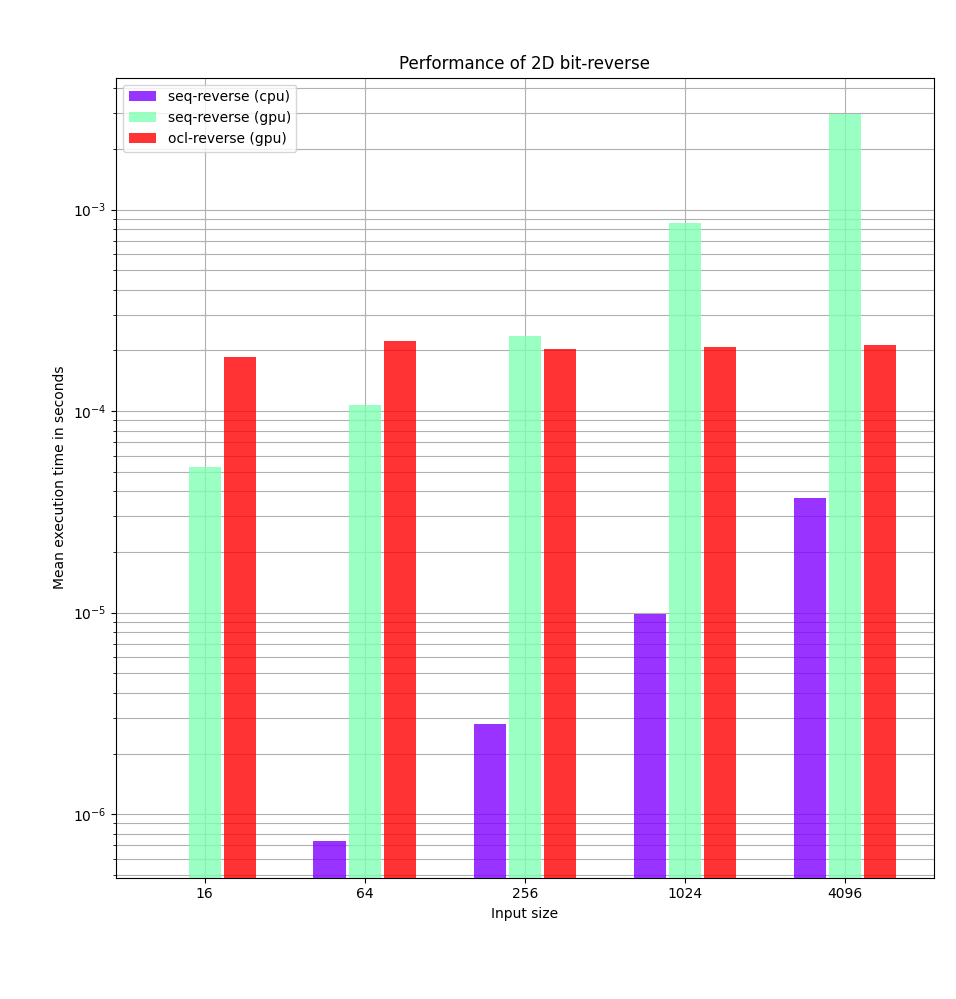
\includegraphics[width=1\linewidth]{resources/images/bit-reverse-cl-low.png}
	\caption{Bit-reversal performance for small input sizes up to 4096 elements.}
	\label{fig:bitrevperf}
\end{figure}

Luckily the performance of the OpenCL bit-reversal is comparatively better for
larger input sizes as shown in figure \ref{fig:bitrevperfh}. The performance
start to gain on the sequential CPU version from around 65000 input elements
and the performance improvement becomes bigger for larger input sizes.

\begin{figure}[h]
	\centering
	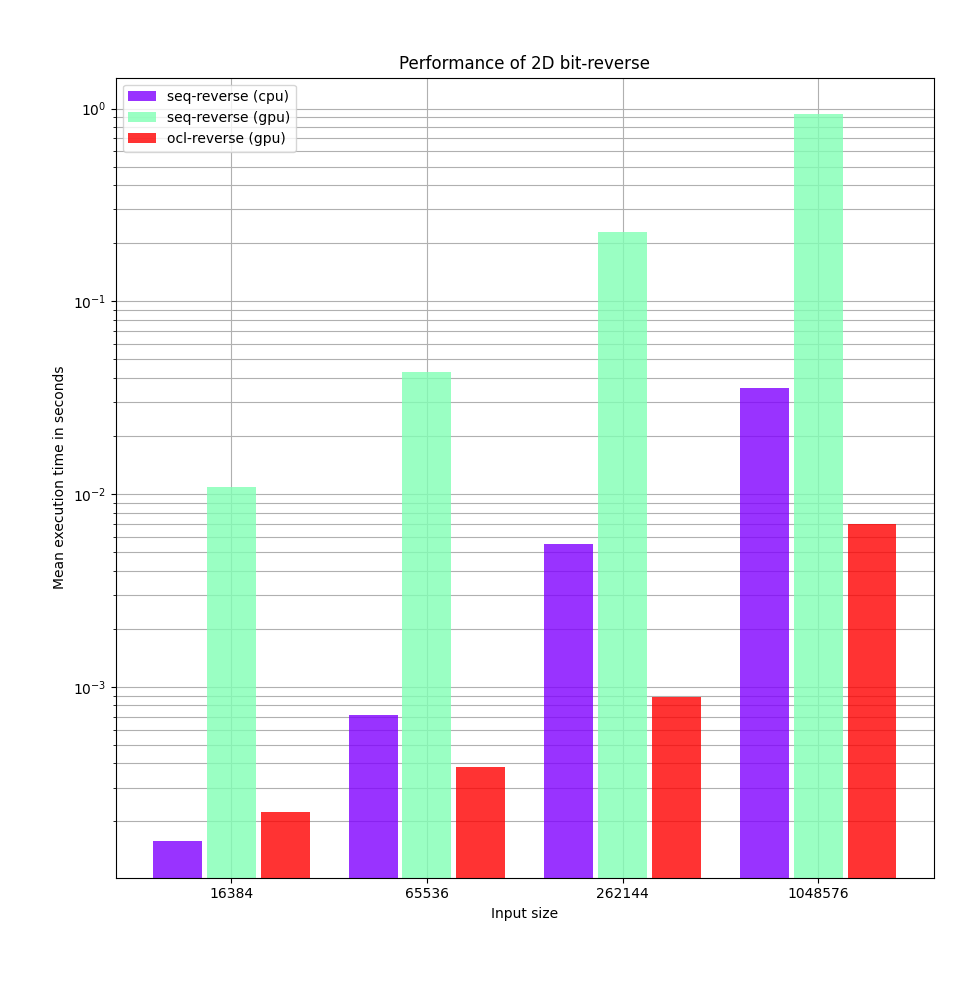
\includegraphics[width=1\linewidth]{resources/images/bit-reverse-cl-high.png}
	\caption{Bit-reversal performance for large input sizes up to 1048576 elements.}
	\label{fig:bitrevperfh}
\end{figure}

Compared to the performance of the the remainder of the FFT algorithm this
bit-reversal is no longer the primary bottleneck. Therefor, the performance of
the bit-reversal at this point is adequate at least until the FFT algorithm
has been improved further. The next section will analyze what parts of the
FFT algorithm have the worst performance in an attempt to optimize them.

\section{Profiling the FFT}

The profiling of OpenCL applications will be done using the
\textit{ROCprofiler} which supports similar performance counters to Nvidia's
\textit{Nsight}. Since the lookup table for the FFT is quite large it is
expected that the bottleneck might be caused due to memory stalls. In order
to establish this the \textit{MemUnitBusy} metric is used. Perhaps local 
memory could be used as the same elements from the lookup table are accessed
multiple times. The performance is profiled using input sizes of 4096 and
1048576 elements as the cache size of this GPU is 16 kilobytes. The lookup
table should occupy $(4096/2)*8=16384$ bytes. The reason for this substantial
difference in input sizes is measure fundamentally different behavior as the
performance impact of the data not fitting in the cache is expected to increase
slowly up to a tipping point were the required execution time starts increasing
drastically. From previous measurements this seems to occur primarily between
262144 and 1048576 input elements. From previous roofline models such as the
one shown in figure \ref{fig:gpuroofline} it became clear that the arithmetic
intensity of the FFT algorithm is low enough that the computation can become
memory bound even with coalesced memory accesses.

The results are visualized using Chromium its tracing function which can be
opened using the \textit{chrome://tracing} url. The first results for the
small input size of 4096 elements are shown in figure \ref{fig:tracesmall}.
From top to bottom the bars represent host activity, copies between host and
device and device activity. The area highlighting illustrated the amount of
time that is taken between launching individual kernel calls. The bottom trace
being much smaller indicates that the overhead of queuing multiple kernels is
limiting the potential performance for these small input sizes, however this
delay is likely due to the profiling itself. For these small trace the
\textit{MemUnitBusy} busy ranges between 0 and 49 were the 49 is seen at the
middle kernel call.

\begin{figure}[H]
	\centering
	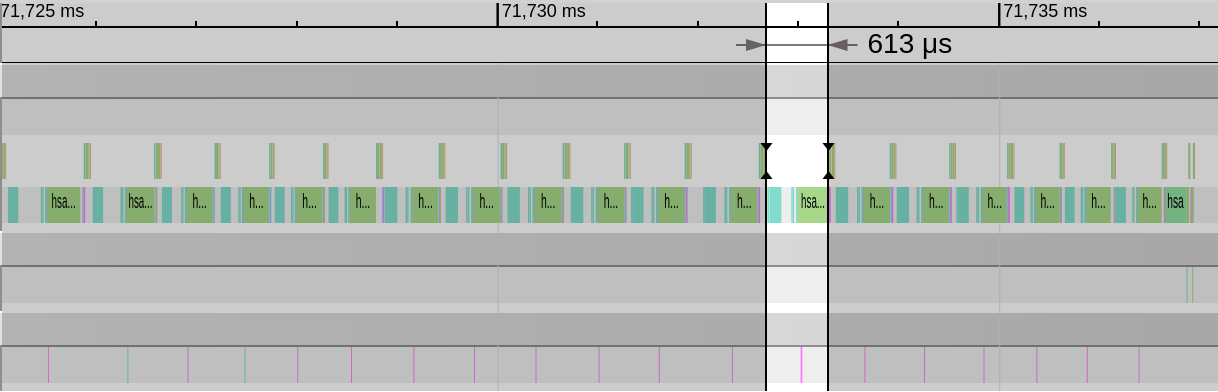
\includegraphics[width=1\linewidth]{resources/images/trace-4096.png}
	\caption{Chrome trace for FFT with 4096 element input size.}
	\label{fig:tracesmall}
\end{figure}

Similarly for the large trace the \textit{MemUnitBusy} is highest for the
middle kernel call but as expected is drastically higher with 97. In total the
\textit{MemUnitBusy} ranges between 63 and 97 indicating that the assumption
that the performance is memory bound is likely correct, especially as at least
five out of the twenty calls at this input size have a \textit{MemUnitBusy}
value of 90 or higher. The trace for this large input size is shown in figure
\ref{fig:tracelarge}.

\begin{figure}[H]
	\centering
	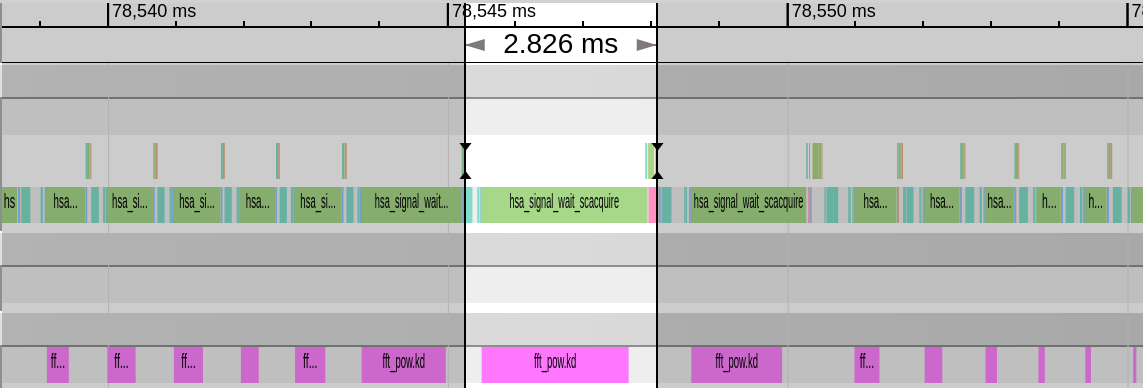
\includegraphics[width=1\linewidth]{resources/images/trace-1048576.png}
	\caption{Chrome trace for FFT with 1048576 element input size.}
	\label{fig:tracelarge}
\end{figure}

For these traces clearly some calls take substantially longer than with the
smaller input sizes with up to 2.8 ms between calls. The minimal delay between 
starting queued kernels seems roughly equal compared to the trace for small
input sizes. Effectively, this indicates the performance can only be improved 
for large input sizes when utilizing local memory, however, this is under the
assumption this delay is still present when not profiling the application.

Unfortunately, the queuing of these kernels can not be prevented as they have
an inherit data dependency and must be executed in this exact order.

\section{FFT Fast-Lookup}

This is the final improvement defined in this work, specifically this
improvement aims to resolve memory stalls due access patterns in the lookup
table for the FFT. Initially, it was envisioned to achieve this by utilizing
local memory, however, this turned out not to be necessary. Instead the
calls to \textit{get\_global\_id()} were changed so they mapped unto different
variables as apparently having the same data accessed by dimension zero instead
of one better coalesces memory accesses. How this was achieved is illustrated
in figure \ref{fig:improvedlayout} were effectively the dimensions for
\textit{get\_global\_id()} with respect to variables \textit{j} and \textit{i}
were swapped.

\begin{center}
	\begin{figure}[H]
		\cexternal{resources/c/new-layout.c}
		\captionsetup{justification=centering}
		\caption{Improved kernel memory access pattern here variable \textit{j}
			first used \textit{get\_global\_id(1)}, contrarily, to \textit{i}
			which used \textit{get\_global\_id(0)}.}
		\label{fig:improvedlayout}
	\end{figure}
\end{center}

With this improved access pattern the performance can be evaluated against
previous FFT implementations as well as against FFTW. This is done in figure
\ref{fig:flkfft} using a logarithmic scale. Please note that all measured
execution times for the FFT algorithms exclude the bit-reversal except for
FFTW as it is not applicable there.

\begin{figure}[H]
	\centering
	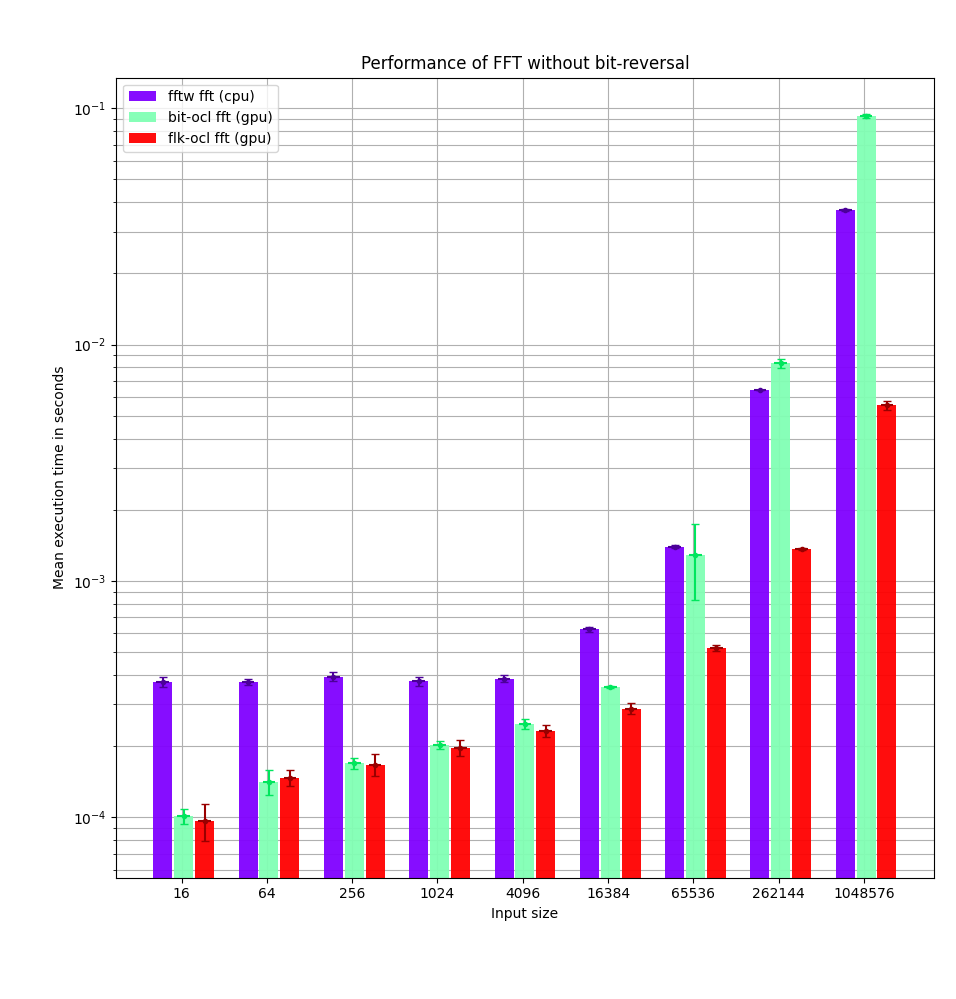
\includegraphics[width=1\linewidth]{resources/images/flk-ocl-fft.png}
	\caption{Performance of different FFT algorithms.}
	\label{fig:flkfft}
\end{figure}

Clearly, this improved access pattern has a large effect on the performance as
The OpenCl implementation now greatly outperforms FFTW for even the largest
input size. As an addition to previous figures the standard deviation is shown
since the variance was quite large for small input sizes. Looking at these
small input sizes it must be true that delay between launching queued kernels
must in part be due to profiling otherwise the performance could never have
improved.

\section{Alternative OpenCL Runtime Targets}

It was envisioned to perform similar performance evaluations for alternative
OpenCL run-time's that utilize the CPU instead of the GPU. Unfortunately,
preliminary results showed that the would provide little insights as the
performance was extremely poor even compared to sequential CPU implementations.
Nevertheless, this section briefly describes the run-time's tested and their
performance at a select amount of input sizes.

Both the pocl\cite{Jskelinen2014} and Intel Xeon run-time's were
evaluated both supporting OpenCL 1.2. Using these run-time's required some
programmatic changes mainly related to the host API. The relevant source code
used for these evaluations can found in the repository with branch
\textit{cl1.2}. However, this conversion from OpenCL 2.0 to 1.2 has only been
applied to the OpenCL bit-reversal implementation. For these evaluations the
input size was limited to 256 elements as this exhausted the entire 32GBs of
working memory off the target hardware. Alternatively, this input size could
have potentially be increased for the Intel Xeon run-time's as these
are evaluated using the DAS5.

At this input size of 256 input elements Intel Xeon took 1.8, 3.5, 1.4 and 1.4
seconds for the windowing, bit-reverse, FFT and magnitude respectively.
Compared to the performance of the ROCm runtime this is at least 20000 times
slower compared to the same implementation. Pocl performed even worse taking
18.7, 38.0, 134.3 and 18.0 seconds for the windowing, bit-reverse, FFT and
magnitude respectively.

If an attempt would be made to optimize the performance using CPU run-time's
a good first step would likely be to ensure the number of work-units launched
matches the number of logical cores.

\section{Future Work}

This work defined how a specific FFT algorithm could be implemented in OpenCL
and defined several improvements to this initial algorithm. This resulted in
the entire computation including memories transfer for up to 1048576 input
elements being computed within 16.66ms. It is believed that this is
considerably decent performance. This is because the same computation using
FFTW takes longer even though both the CPU and GPU used to evaluate the
performance have comparable peak FLOPS/s. As a final figure the speed-up
compared to the first OpenCL implementation is shown in figure
\ref{fig:speedup}. Undeniably, the choice of stacked bargraph with a
logarithmic scale is very poor as it makes extremely difficult to estimate the
speedup of the FFT as the bit-reverse dominates the bar due to its relative
size. Unfortunately, this graph could not be improved due to time constraints.

\begin{figure}[h]
	\centering
	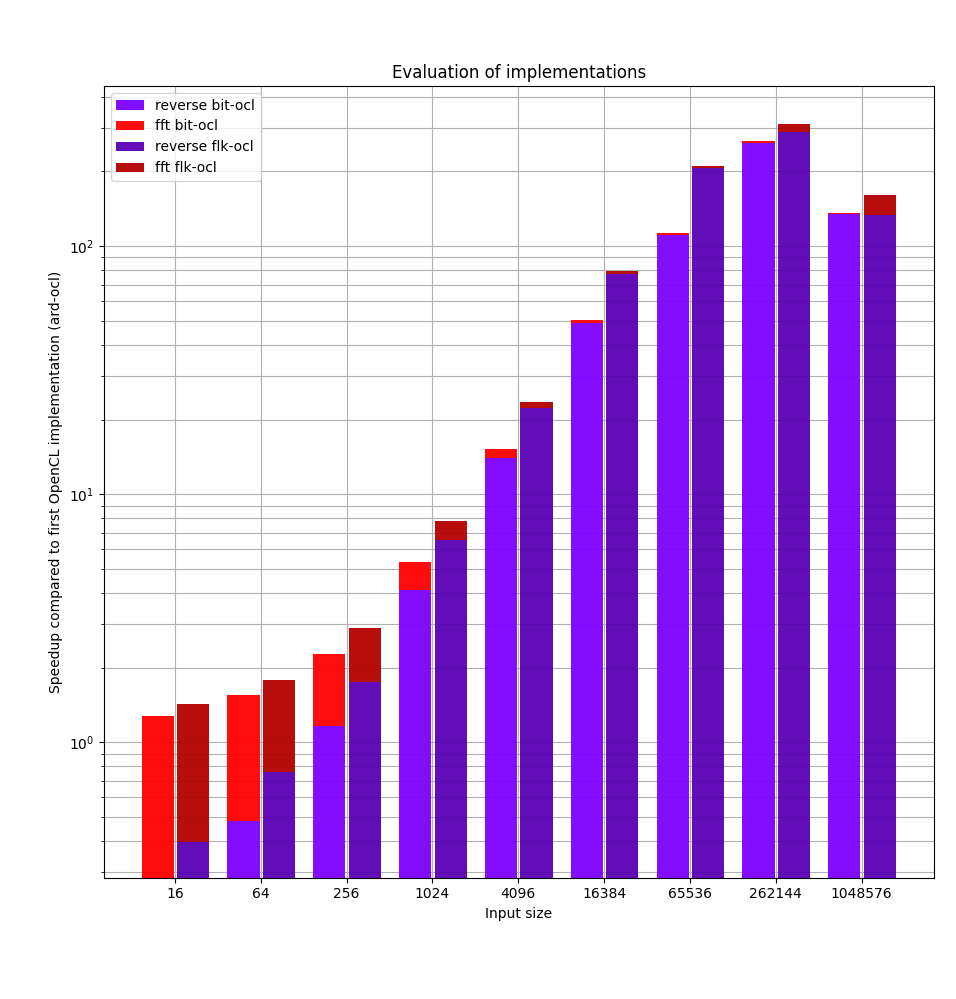
\includegraphics[width=1\linewidth]{resources/images/overal-speedup.png}
	\caption{Speedup of OpenCL implementations compared to first OpenCL
		implementations. Only altered parts of the computation are
		illustrated.}
	\label{fig:speedup}
\end{figure}

However, some of the optimizations introduced further constraints on the
input size. The primary cause of this constraint is due to the bit-reversal
algorithm which requires to place all input elements in a 2D matrix, thereby,
requiring the input size to be evenly divisible by two. It is believed that
this constraint can be removed by choosing the largest possible grid size so
that another grid square of equal size can be added below it. Effectively this
will turn the square into a rectangle. For instance for an input size of 32
elements this would create two four by four squares turned into a four by eight
matrix.

Another possible further improvement can be achieved by condensing the lookup
table used on the device. This is because every lookup table will effectively
contain all the elements for the previous power of two. However, the formula
to compete the index between these different powers of two is non-trivial.

Alternatively, to further optimizing the current algorithm OpenCL 2.0
introduces many new algorithms which previously could not be executed on the
GPU. This is because OpenCL 2.0 introduces nested parallelism which effectively
allows to perform recursive algorithms on OpenCL devices. Particularly the
traditional Cooley-Tukey recursive FFT and the
Elster-Huff-Strandh\cite{Elster2009} bit-reversal would be interesting
algorithms.

Clearly, FFT algorithms for OpenCL devices is a research topic that is not
fully explored yet.

\addcontentsline{toc}{section}{\protect\numberline{}TERMINOLOGY} 
\section*{TERMINOLOGY} \label{term}

This section hopes to define some common terminology as well as clearly detail
how some of these terms are interpreted. Mainly this section serves to avoid
confusion.

\begin{enumerate}
	\item GPGPU - Used as a term to refer to the graphics card that is
	typically used for 3D graphics but in this context used for more general 
	computation. Sometimes simply referred to as \textit{device}, however, this
	term is used in a more general sense. Refers to both the act of using a GPU
	as well as a specific GPU used for general purpose computations.
	\item Runtime - Used as term to describe an implementable standard that
	allows for the execution of applications. Typically, these standards expose
	a well defined API, additionally, the target hardware is generally
	unavailable without such a runtime implementation. The fundamental
	difference between libraries, frameworks and run-time's is that only
	run-time's enable specific hardware to be used.
\end{enumerate}

\bibliographystyle{IEEEtran}
\bibliography{bibliography}

\end{document}